\chapter{走进化学世界}

化学就是研究\uline{物质}及其\uline{变化},它不仅研究已经存在的物质,还
要研究和创造自然界原本不存在的新物质。例如,半导体材料,电阻几乎为零的
超导体,有记忆能力的新材料,等等。

化学在保证人类生存和提高生活质量上有很大帮助。例如:

\begin{itemize}
\item 化肥和农药,增加粮食产量。
\item 化学合成药物,指抑制细菌和病毒。
\item 化学新能源、新材料。
\end{itemize}

近代化学突破源于两点:

\begin{enumerate}
\item 物质是由分子原子构成的,分子中原子的重新组合是化学变化的基础。
\item 元素周期表。
\end{enumerate}

这两个突破使得化学研究有迹可寻。化学的科学定义:\textbf{化学是在分子、
  原子层上研究物质\uline{性质、组成、结构}与\uline{变化}规律的科学}。研
究物质是指研究其性质、组成和结构等\uline{静态特征},而变化是化学反应,
也即原子的重新组合,这是一个\uline{动态过程}。

\section{性质及变化}

物质变化分两两种:

\begin{itemize}
\item 物理变化:没有生成新物质的变化,如物质形态发生变化。气态、液态、
  固态三态之间的相互转换的过程就是物理变化。
\item 化学变化或叫化学反应:生成新物质的变化(原子重新组合),常表现为
  颜色变化,放出气体,生成沉淀等。化学变化还伴随物质能量变化,如吸热、
  放热、发光等。
\end{itemize}

虽然物理变化也通常伴随能量转换,但主要借用外部能量。而化学变化和能量可
以只来自物质本身,不需要外部能量辅助。

依据物质变化过程中表现出的性质,可有:

\begin{itemize}
\item 化学性质:物质在化学变化中表现出的性质。例如,铜在潮湿的空气中生
  成铜绿。
\item 物理性质:物质不需要化学反应就表现出来的性质。物质颜色、状态、气
  味、硬度、熔点、沸点、密度等都是物理性质。例如,常态下,氧气是种无色、
  无味的气体。注意,物理性质可能是物理变化过程表现出的性质,如物质的三
  态。
\end{itemize}

外界条件改变时,物质性质也会随着变化,因此,描述物质性质时往往\uline{要
  注明条件}。如,当温度升高时,固态冰变成液态水,再加温,水会沸腾。液体
的沸点是物理性质,但受大气圧强的影响。大气稀薄的地方,大气圧强变小,这
时水的沸点会降低,容易烧开。

\subsection{大气圧}

由于大气圧强是变化的,人们把 $1 atm = 101 kPa = 76 cm \text{水银柱重
  量}$当作标准大气圧强。大气压强是指大气对浸在它里面的物体产生的压强,
也叫大气圧或气圧,可以用空气的重力或分子热运动来解释其产生机理,而且这
两种解释是等价的。

那么如何用重力和分子热运动解释呢?在密封空间内,气圧的产生应从微观上来
解释。气体分子热运动时,撞击空间内壁,产生作用力(内壁也同时产生反作用
力),这个作用力就是气体圧力。没有内壁就不会产生气体圧力!圧强是单位面
积上的圧力,表示强度,不用考虑内壁的存在。

由于分子作用力各向同性,所以任一点的圧强在不同方向上相同。

对于空气呢?空气分子同样作热运动,但是没有内壁,怎么产生圧力呢?有地球
引力!地球引力相当于上述密闭空间内壁的反作用力。所以空气中任意一点也有
空气圧力,进而也有圧强。同理,空气圧力也是各向同性的。

至于圧强的数值计算,两种情况有所不同,关键是算出分子热运动的作用力。对
于密闭空间,它是 $P = nTR/volume$. 对于空气,因为重力和空气分子热运动产生
的撞击力平衡,大气压强是大气施加于单位面积上的重力,即该地单位面积垂直
向上延伸到大气层顶的空气柱的总重力。简单的数学公式是 $P = m \cdot
g/area$. 实际中要考虑不同高度处重力加速度 $g$ 的不同。

\section{化学实验}

\subsection{注意事项}

\begin{itemize}
\item 手不接触药品,不尝药品,鼻孔不可太靠近瓶口(特别是气体)。
\item 实验剩余药品不能放回原瓶,不能随意丢弃,不能带出实验室。要放入指
  定容器。
\item 节约药品。未说明剂量时,液体一般取 $1 - 2 \, mL$, 固体只需盖满试
  管底部即可。
\item 保护眼睛,如果进了药液,应立即用清水清洗,要眨眼睛。
\end{itemize}

\subsection{药品取用}

\begin{itemize}
\item 固体:广口瓶。药匙(粉状、颗粒)、摄子(块状),取完应擦净。玻璃
  容器横放,块状放容器口,缓缓坚立,滑入底。药匙送粉状入试管底,再直立。
\item 液体:细口瓶。倾倒法。瓶塞倒立桌面,瓶口紧挨试管口,瓶身标签面朝
  手心。定量取液,用量筒。量液时,视线与凹液面最低处保持水平。仰视偏多,
  俯视偏少。取少量液体用滴管,应保持橡胶帽朝上,不可平放、倒放,否则腐
  蚀橡胶帽或污染试剂。滴管应悬空滴液,不可接触容器口,否则因为试剂太
  少,沾在内壁。用完即洗。
\end{itemize}

\subsection{物质加热}

一般用酒精灯。不可以向燃着的酒精灯添加酒精,也不可以用一个点燃另一个。
用灯帽熄灭,不可用嘴吹。熄灭后,取下灯帽再盖上。

加热试管液体:

\begin{enumerate}
\item 试管外壁应干燥,液体不超过容积的 1/3.
\item 试管夹由试管底部套上、取下。
\item 先使试管底部均匀受热,再用外焰固定加热。
\item 试管口不要对着自己或他人。
\item 加热后的试管不能立即接触冷水或用冷水冲洗。
\end{enumerate}

\subsubsection{三层火焰}

本节顺便说下蜡烛然烧问题。蜡烛然烧时,蜡固体先熔化、气化,再与空气中氧
气发生化学反应。

外焰是红白色,温度高;而内焰为红色且边缘是蓝色,温度低。焰心没有发生燃
烧,所以不烧手。温度的高低主要由与氧气接触面积决定。外焰处氧气最多,燃
烧最充分,温度最高。焰心处氧气已消耗殆尽,所以没有燃烧。

\uline{色温}和\uline{温度}是两个不同的概念。色温反应的是单个分子的能量,
能量越高,颜色越偏蓝。温度是分子热运动的宏观测量,不仅要考虑单个分子能
量,还应考虑分子总个数。在相同分子个数情况下,蓝焰温度肯定比黄色或红色
高。

但在蜡烛然烧时,外焰温高除了氧气多外,和热气体上升也有关系。另外,既然
外焰燃烧更充分,为何不见蓝色。实际是有蓝色的,只是被遮住了。外焰处蜡蒸气
非常多,被外焰加热后,变成白炽色,把燃烧的蓝色吸收了。所以外焰的高温不
是因为黄色,而是蓝色(充分燃烧)和上升热气。

\subsection{仪器连接}

玻璃管,胶皮管,橡胶塞:

\begin{enumerate}
\item 玻璃管和橡胶塞:玻璃管口用水湿润,对准橡胶塞上的孔稍用力转动、插入。
\item 玻璃管和胶皮管:玻璃管口用水湿润,稍用力即可插入。
\item 容器口和橡胶塞:慢慢转动橡胶塞,塞入容器口(如试管)。
\item 气密性检查:用手握紧试管,观察水中导管口是否有汽泡冒出,有则好。
\end{enumerate}

\subsection{洗涤玻璃容器}

必需洗涤玻璃容器,否则影响实验效果。以洗试管为例:

\begin{enumerate}
\item 倒掉废液。
\item 注入半试管水,振荡后再倒掉。
\item 重复上一步聚。
\item 如试管内壁还有不易洗掉残留物质,用试管刷刷洗。洗刷时,须转动或上
  下移动试管刷。
\end{enumerate}

洗过的玻璃容器内壁附着的水既\uline{不聚成水滴,也不股下流},表明仪器已
洗干净。

\chapter{空气}

\section{简介}

空气的主要成分是氮 78\%, 氧 21\%, 稀有气体 0.94\%, 二氧化碳 0.03\%, 其
它气体和杂质占 0.03\%. 其中氮和氧几乎各占 1/5 和 4/5. 稀有气体主要是氦
hài, 氖、氩、氪、氙 xiān, 氡等。
                     
\begin{itemize}
\item 混合物:由两种或两种以上的物质混合而成的物质。组成混合物的各种成
  分保持着它们各自的性质。
\item 纯净物:只有一种物质组成。纯净物可以用\uline{化学式}表示,如氮气
  是 \ce{N2}, 磷是 \ce{P}, 五氧化二氮是 \ce{P2O5} 等。
\end{itemize}

\section{成分}

各主要成分。












\chapter{物质列表}

\begin{table}[!htb]
  \centering
  \begin{tabular}[!htb]{r|c|c}
    \toprule
    \diagbox{化学式}{叁数} & \text{名称、别名} & \text{颜色和状态} \\
    \midrule
    \ce{CuSO4} & 硫酸铜、胆矾、蓝矾 & (无水)灰白色粉未、(有水)
    蓝色结晶固体 \\
    \ce{H2O} & 水 & 无色液体 \\
    \ce{KAl(SO4) * 2H2O} & 十二水合硫酸铝钾、明矾 & 无色或白色的八面体晶体 \\
    \ce{Fe} & 铁 & 银白色固体 \\
    \ce{Al} & 铝 & 银白色固体 \\
    \ce{O2} & 氧气 & 无色无味气体 \\
    \bottomrule
  \end{tabular}
  \caption{常见物质列表}
  \label{tab:common-substances}
\end{table}


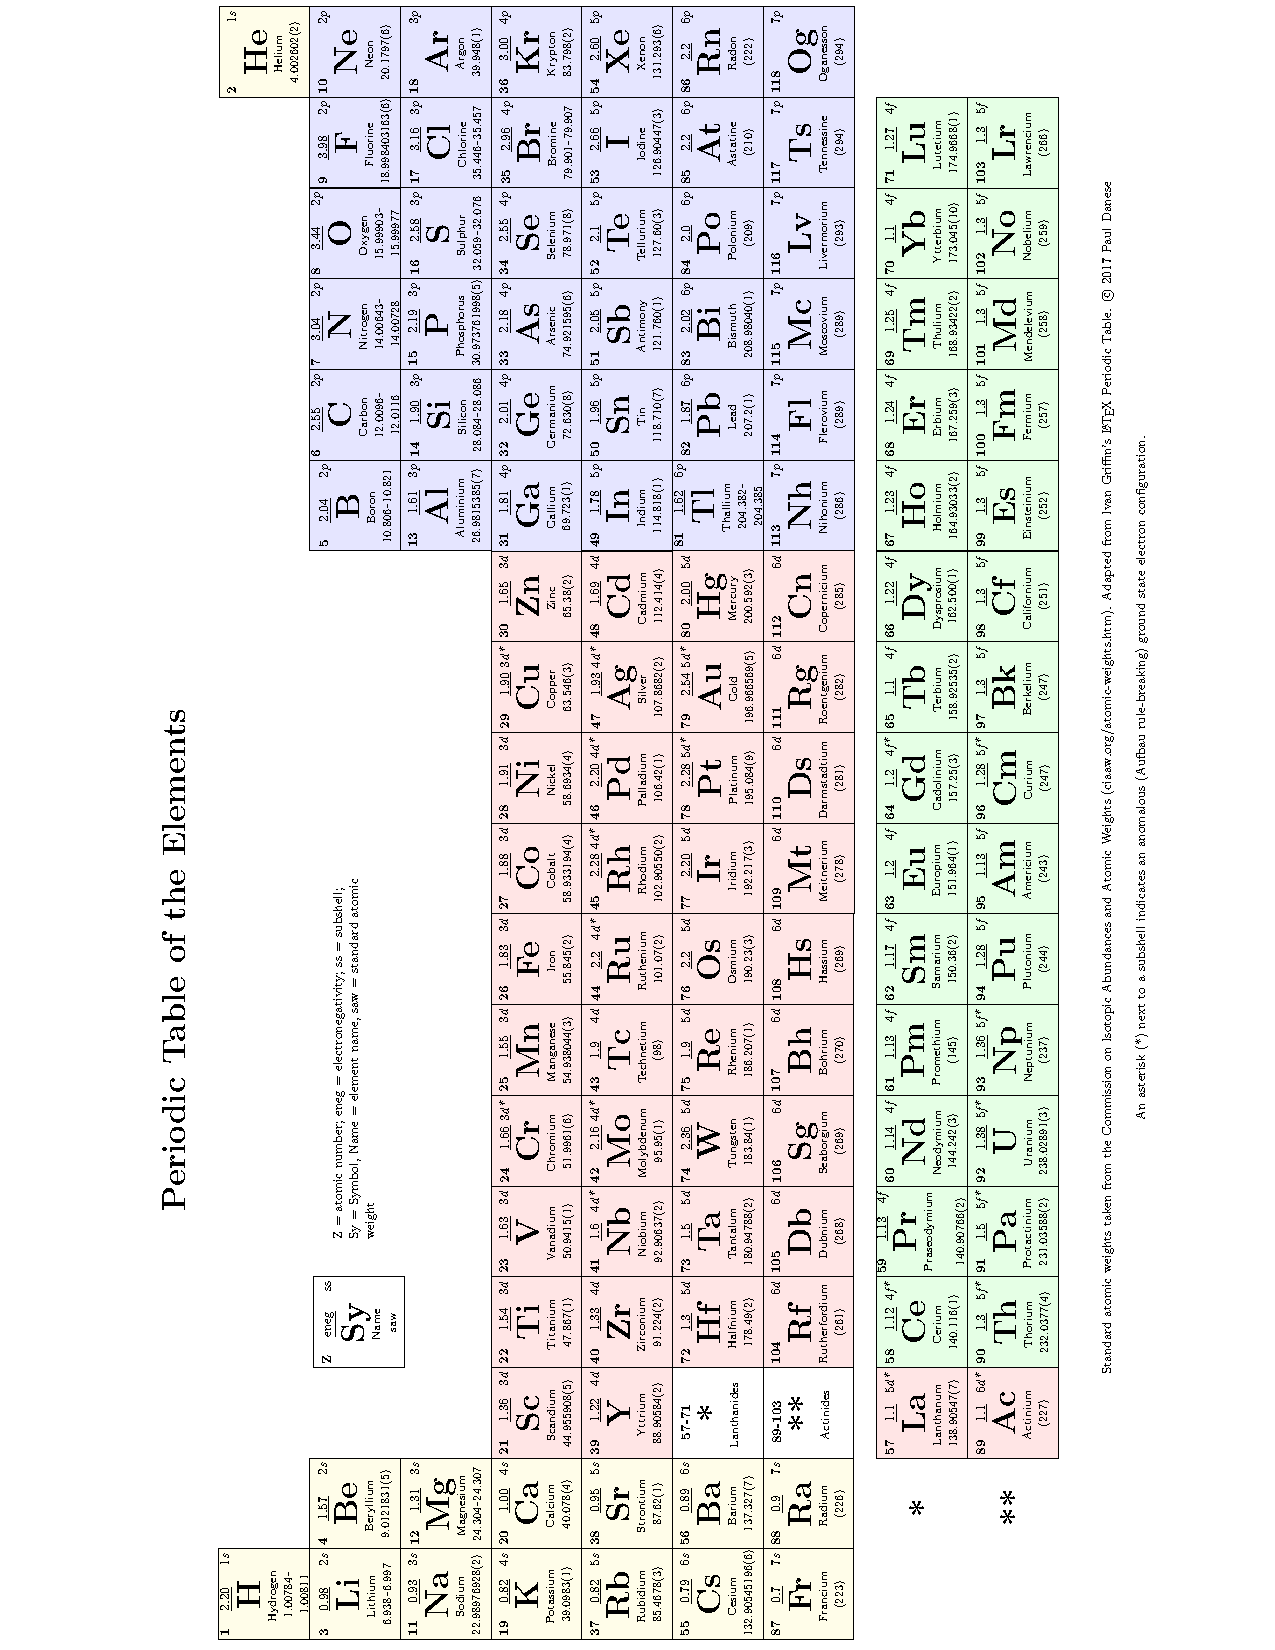
\includepdf[pages=-]{periodic_table.pdf}
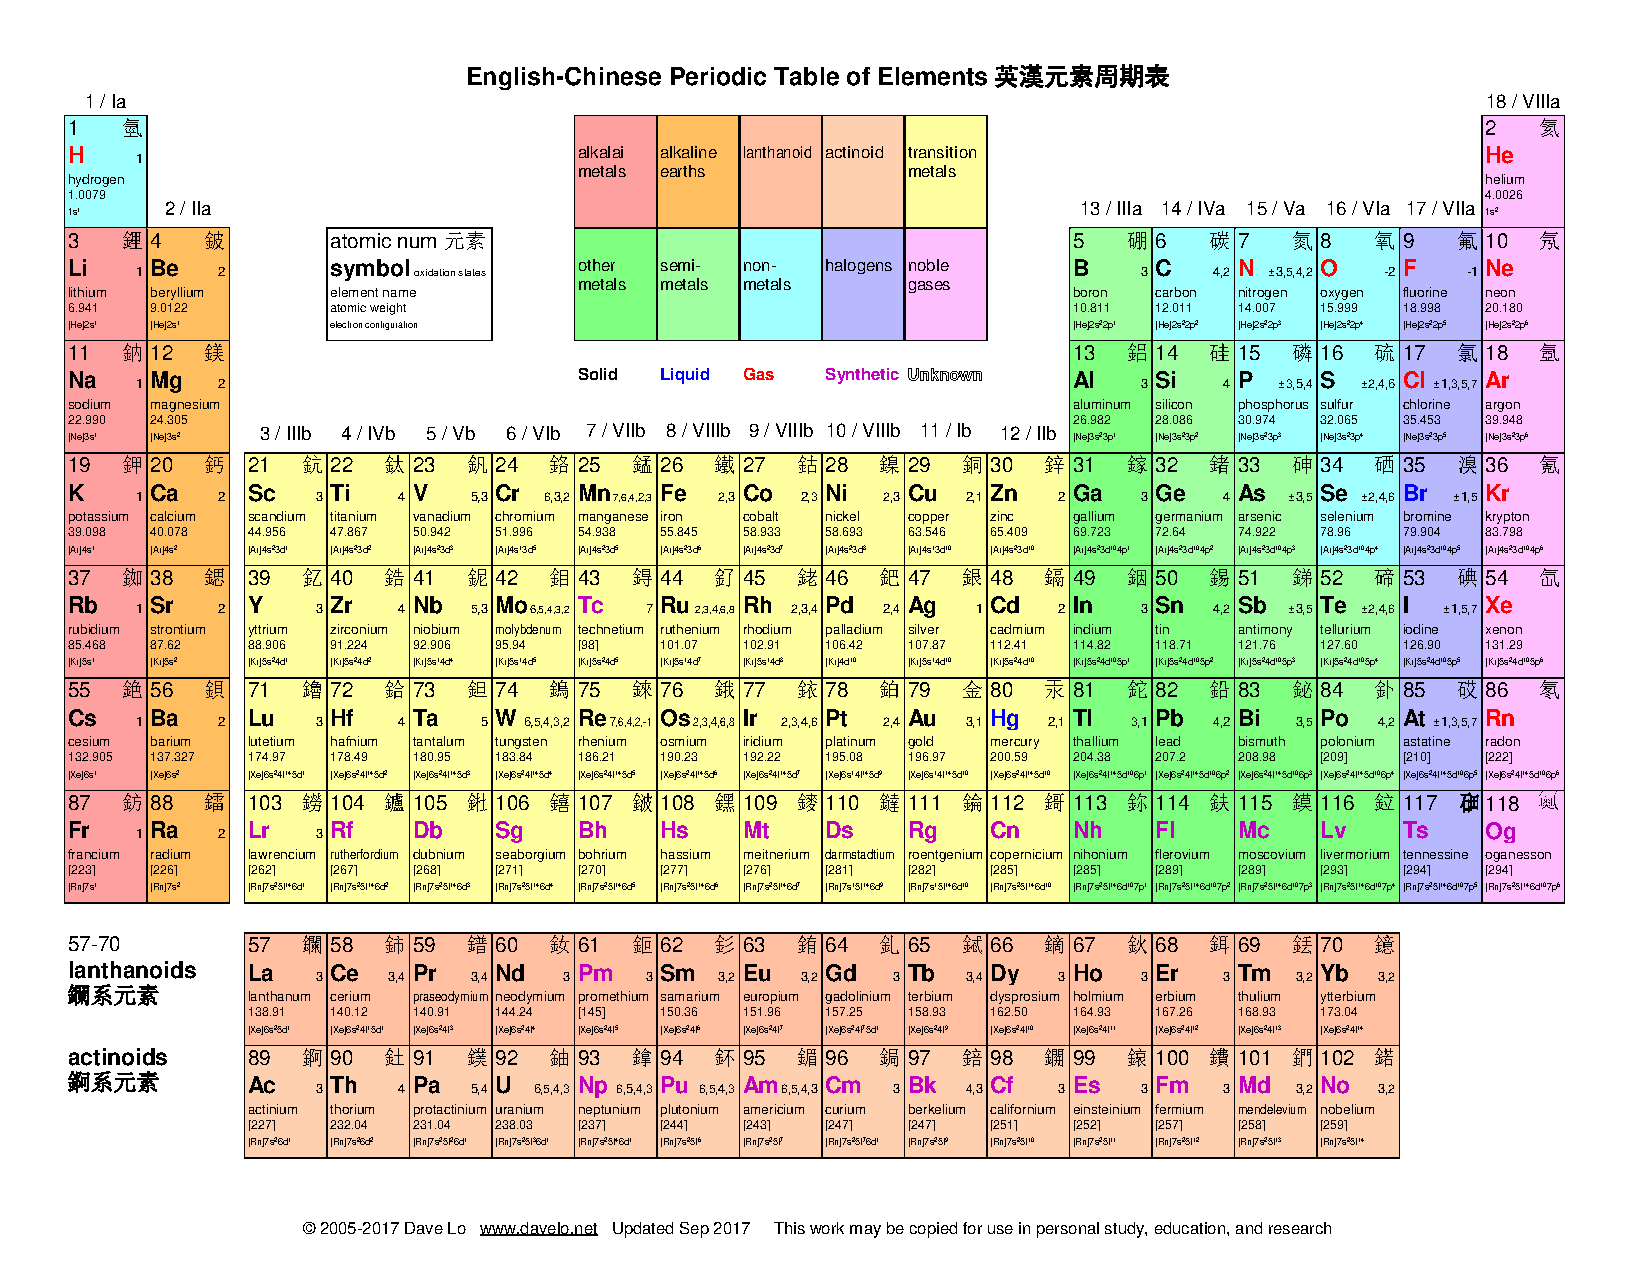
\includepdf[pages=-]{periodic_table_tra.pdf}


%%% Local Variables:
%%% mode: latex
%%% TeX-master: "main"
%%% End:
